\documentclass[aps,pra,twocolumn,amsmath,amssymb,nofootinbib,superscriptaddress]{revtex4}

\newcommand{\bra}[1]{\langle#1|}
\newcommand{\ket}[1]{|#1\rangle}
\newcommand{\op}[2]{\hat{\textbf{#1}}_{#2}}
\newcommand{\dagop}[2]{\hat{\textbf{#1}}_{#2}^\dag}
\newcommand{\keith}[1]{{\color{cyan}{#1}}}
\newcommand{\peter}[1]{{\color{blue}{#1}}}
\newcommand{\remove}[1]{{\color{red}{#1}}}

\usepackage[pdftex]{graphicx}
\usepackage{mathrsfs}
\usepackage[colorlinks]{hyperref}
\usepackage{braket}

\begin{document}

\bibliographystyle{apsrev}

%
% Title
% 

\title{An introduction to boson-sampling}

%
% Authors
%

\author{In no particular order}

\author{Peter P. Rohde}
\email[]{dr.rohde@gmail.com}
\homepage{http://www.peterrohde.org}
\affiliation{Centre for Engineered Quantum Systems, Department of Physics and Astronomy, Macquarie University, Sydney NSW 2113, Australia}

\author{Bryan Gard}

\author{Keith R. Motes}

\author{Jonathan P. Dowling}

\date{\today}

\frenchspacing

%
% Abstract
%

\begin{abstract}
\end{abstract}

\maketitle

\section{Introduction (Bryan)}

\subsection{Motivation for linear optics quantum computing and boson-sampling}

To-date, many different physical implementations and models for quantum computing have been proposed. These implementations include atom and ion trap quantum computing, superconducting qubits, nuclear magnetic resonance, quantum dots, nuclear spin, and optical quantum computing. When describing an implementation, one can use various models of computation. These include the gate model, cluster (or graph) states \cite{bib:Raussendorf01, bib:Raussendorf03}, topological, adiabatic, quantum random walks \cite{bib:ADZ}, quantum Turing machines, permutational, and the one-clean qubit models (\textbf{PLEASE ADD REFERENCES FOR EACH OF THESE}). The most familiar and intuitive model is the gate model as it is most analogous to the classical circuit model of computation. We use this gate model in order describe linear optics quantum computing (LOQC) and eventually a special purpose subset, boson-sampling.

As stated, there exist many choices of implementations and computational models. Certain pairs of choices certainly have natural synergy but a fair question to ask is, which choice is likely to yield the first implemented quantum computer? The answer is likely not just one choice, but a composite of different choices for the various required components of a quantum computer. For this discussion we focus on LOQC for its main allure of `simple' implementation.

There is a many year history in the physics community of investigations into the use of linear interferometers, particularly linear optics interferometers, as a type of quantum information processor. However in most of this early research the conclusion was that a linear optics interferometer (alone) could not be used to make a universal quantum computer, regardless of the input states. For example in 1994, one year before Shor's discovery of the now-famous quantum factoring algorithm, there appeared a paper by {\u C}ern{\' y} that proposed to use a linear interferometer to solve \textbf{NP}-complete problems in polynomial time, but the scheme suffered from an exponential overhead in energy \cite{cerny}. Along the same lines, in 1996, Clauser \& Dowling showed that a linear optics Talbot interferometer could be used to factor integers in polynomial time but with either an exponential blow up in energy or physical size \cite{clauser}. Then, also in 1996, Cerf, Adami \& Kwiat showed how to construct a programmable linear optics interferometer that could perform any universal logic gate with single photon inputs but this scheme too suffered an exponential overhead in spatial dimension. In 2002 Bartlett \emph{et al.} showed that even with quadratic nonlinearities any interferometer that processes only Gaussian state inputs can be efficiently simulated classically, a continuous variable analog of the Gottesman-Knill theorem for discrete variables in the ordinary circuit quantum computation model \cite{bart}. 

This litany of `no-go' theorems led to the widespread belief that linear interferometry alone could not provide a path to universal quantum computation and that, as a corollary, all linear optics interferometers are efficiently simulateable on a classical computer. For completeness we will introduce the LOQC approach of Knill, Laflamme \& Milburn (KLM) \cite{knill,kok} in the following section, but the remaining focus of this chapter is instead on boson-sampling. That is because the KLM scheme set of universal gates requires intermediate measurements on ancilla photons with a feed-forward mechanism that imparts a type of effective Kerr nonlinearity on the system \cite{lap}. We explicitly only discuss linear optics implementations due to the fact that nonlinear Kerr media exhibit very poor efficiency for our purposes \cite{nielsen}, and present-day Kerr mediums exhibit only very weak non-linearities.

Hence it came as a surprise to many of us in the quantum optics community when Aaronson \& Arkhipov (AA) argued that, in general, the operation of a passive linear optics interferometer with Fock state inputs can very likely not be simulated by a classical computer \cite{aar}. In particular if one considers a sampling of the outputs, utilizing photon-number discriminating detectors, such a boson-sampling device cannot be predicted with a classical computer without an exponential overhead. This has become known in the computational complexity community as the boson-sampling problem. 

The conclusion that computing the output of a linear optics interferometer with Fock state inputs is likely a computationally hard problem was independently reached by Gard \emph{et al.}, in the context of trying to compute the related problem of multi-photon coincidence counts in the output of a linear optics interferometer implementation of a quantum random walk with multi-photon walkers \cite{gard2}. In follow up papers, Gard \emph{et al.} \cite{gard}, as well as Motes \emph{et al.} \cite{motes}, argued from a physical (as opposed to computational complexity) point of view that this inability to simulate such interferometers arose from two necessary requirements: (1) The photons `interact' at the beamsplitters via a Hong-Ou-Mandel effect that gives rise to an exponentially large Hilbert space in the number-path degrees of freedom that rules out a brute force simulation of the interferometer; and (2) That the simulation of the interferometer is also tied to the need to compute the permanent of a large matrix with complex entries, a problem known to be in the complexity class \textbf{\#P}-complete, that is thought to be an intractable problem not only classically but even on a universal quantum computer \cite{bib:Ryser63}. The reason for the second requirement is that, due to the Gottesman-Knill theorem, it is known that there are examples of quantum circuits with gates all in the Clifford algebra class that generate exponentially large amounts of qubit entanglement but are nevertheless and surprisingly classically simulateable. Sometimes there are shortcuts through the exponential Hilbert space and so by tying the simulation to the problem of the permanent solving we make is very unlikely that any such shortcuts exist. For example, the equivalent sampling problem with fermions rather than bosons is known to be classically easy to simulate, as the problem relates to matrix determinants rather than permanents, which are known to be in the complexity class \textbf{P} (\textbf{CITATION FOR FERMION SAMPLING}).

Since the first appearance of the AA paper in 2010 there has been an explosion of research into the field of boson-sampling. As we will discuss below there have been a number of experiments utilizing three photons from spontaneous parametric down conversion (SPDC) sources \cite{ralph,broome,spring,anon,till,crespi} (although these experiments are under debate as not all three photons were heralded single photons \cite{bib:dowlingSchmampling}). The experimental work has continued in parallel to a number of theoretical developments considering the effects of loss, noise, decoherence, non-Fock inputs, scalability of SPDC sources, ion-trap implementations, and so forth \cite{rohde1,rohde2,jiang,motes,shch}. We will discuss and summarize these results and more in the sections below. 

So then there come the questions -- why is boson-sampling getting so much attention and what is it good for? The answer is that boson-sampling is a new example of a computationally complex mathematical problem that cannot be simulated on a classical computer, but which significantly reduces experimental requirements compared to universal quantum computing schemes. The appeal is that this is the first interesting example of a non-trivial quantum computing paradigm to be proposed in some while and the true scope and power of such machines is not yet fully understood. 

Then the question arises; what is a boson-sampling machine good for other than boson-sampling? The boson-sampling problem itself, other than being a computational curiosity, has no known practical applications or `killer apps' such as we find with the Shor factoring algorithm. But prior to 1994, when the Shor algorithm was invented, there the same question was asked; `What is a quantum computer good for?' Feynman's work in the 1980s had hypothesized that an ordinary quantum computer could be used to carry out certain physics simulations without the exponential overhead required to do so on a classical computer but this hypothesis was not proved until Lloyd's work in 1996 \cite{feyn,lloyd}. The first non-trivial application for an ordinary quantum computer was the Deutsch-Jozsa algorithm discovered in 1992, but this problem also had no practical applications \cite{deutsch}. So in many ways the boson-sampling quantum computer is like the ordinary circuit-based quantum computer pre-Shor. We have one example of an exponentially hard mathematical problem that the machine can solve but not one that is known to be useful for anything. The lure is that perhaps the linear optics interferometers, now that this hidden computational power has been uncovered, are good for something else besides the boson-sampling problem. This potential is what has captured the imagination of researchers in the field. As we arrive at our boson-sampling scheme by way of LOQC, we still maintain several of its benefits. These include no requirements for excessive cooling of the optical elements, long coherence times compared to the basic gate operations, and relatively simple to understand noise sources.

One final caveat; In almost all papers on the topic of boson-sampling the interferometer is described as a linear device with non-interacting bosons: photons in this case. However the Hong-Ou-Mandel effect (followed by a projective measurement) imparts an effective nonlinearity and hence an effective interaction at each beamsplitter. The presence or absence of a photon in one input mode radically changes the output state that a second photon in the other input mode will find itself in. This `interaction' between indistinguishable particles, known as the exchange interaction, arises simply from the demand that the multi-particle wavefunction be properly symmetrized. While not a force in the usual sense it can give rise to quite noticeable effects. For example, the bound state of the neutral hydrogen molecule, the most common molecule in our Universe, arises from just such an exchange interaction. It is therefore a misnomer to describe these interferometers as linear devices with non-interacting bosons. The exchange interaction is just as real as tagging on an additional term in a Hamiltonian and if one adds postselection in the number basis to the mix this imparts an effective Kerr-like nonlinearity between the bosons to boot.   

\subsection{Introduction to linear optics quantum computing}
 
 We begin by defining some terminology and notation. The smallest amount of data that we can deal with in quantum computing, analogous to the classical computing bit, is the quantum `qubit'. A qubit is defined as 
\begin{eqnarray}
 \left[ \begin{array}{l}
1 \\
0 \\
\end{array} \right] = \ket{0},
\left[ \begin{array}{l}
0 \\
1 \\
\end{array} \right] = \ket{1}
\end{eqnarray}
for a zero and one qubit, respectively. One of the advantages of quantum computing over classical computing is, of course, the ability to use quantum effects. One of these effects is the ability to have a qubit in a superposition of zero and one, that is, in general
\begin{equation}
\ket{\psi} = \cos\left(\frac{\theta}{2}\right) \ket{0} + e^{i \phi} \sin\left(\frac{\theta}{2}\right)\ket{1},
\end{equation}
 and with a specific choice for $\theta =\frac{\pi}{2}$ and $\phi =0$ we can simplify this to
\begin{equation}
\ket{\psi}= \frac{1}{\sqrt{2}} \ket{0} + \frac{1}{\sqrt{2}} \ket{1}.
\end{equation}
This superposition represents that our state, once measured, has a 1/2 probability of being in state zero and a 1/2 probability of being in state one. These superpositions can also be depicted on the Bloch sphere as shown in Fig.~\ref{fig:Bloch}. One may initially want to view these superpositions as being in both states at once and while this idea is true, it is somewhat as once we measure this superposition state, it always takes either the value of zero or one. Before we measured the state however, we of course do not have any information about the state. It is the act of our measurement that forces the state to `choose' a zero or one. Thus there is an attribute of these superposition states to contain some `hidden' quantum information.
\begin{figure}[bt]
 \centering
  %\includegraphics[height=5.25cm]{Bloch.ps}
  \caption{ Bloch sphere showing a way to visualize the rotations that the Pauli matrices apply to a state. Pure states lie on the sphere while mixed states are contained within the sphere.}
  \label{fig:Bloch}
\end{figure}

 Also analogous to classical computing, we need a set of logic gates to perform operations on our quantum states \cite{nielsen}. Some of the most common gates are defined as
\begin{eqnarray}
\textrm{Controlled-NOT (CNOT):} && \frac{1}{\sqrt{2}}\left[ 
\begin{array}{cccc}
1 & 0 & 0 & 0 \\
0 & 1 & 0 & 0 \\
0 & 0 & 0 & 1 \\
0 & 0 & 1 & 0 \\
\end{array} \right] \\ \nonumber
\textrm{Hadamard (H):} &&  \frac{1}{\sqrt{2}}\left[ 
\begin{array}{cc}
1&1 \\
1&-1 \\
\end{array} \right] \\ \nonumber
\textrm{Pauli-X ($\sigma_x$):} && \left[
\begin{array}{cc}
0&1\\
1&0\\
\end{array} \right] \\ \nonumber
\textrm{Pauli-Y ($\sigma_y$):} && \left[
\begin{array}{cc}
0&-i\\
i&0\\
\end{array} \right] \\ \nonumber
\textrm{Pauli-Z ($\sigma_z$):} && \left[
\begin{array}{cc}
1&0\\
0&-1\\
\end{array} \right] \\ \nonumber
\textrm{Phase:} && \left[
\begin{array}{cc}
1&0\\
0&i\\
\end{array} \right] \\
\frac{\pi}{8}: &\;& \left[
\begin{array}{cc}
1&0\\
0&e^{i \pi/4} \\
\end{array} \right]. \nonumber
\end{eqnarray}
The first of these, the CNOT gate, is a maximally entangling two-qubit gate, which is the quantum equivalent of the classical XOR gate, whilst the latter gates are single qubit gates, which implement rotations on the Bloch sphere. The single qubit gates may be trivially implemented using waveplates in quantum optics, whilst the CNOT gate is far more challenging, requiring an effective Kerr non-linearity.

These gates form one choice of a universal gate set. Any choice for a universal gate set can approximate any other gate set to arbitrary precision. In broad terms there are three classes of problems to which quantum computation outperforms classical computing. These classes include algorithms that make use of the quantum Fourier transform such as Shor's algorithm for factoring and discrete logarithms. For $ N=2^n$ numbers, a classical fast Fourier transform would require $ N \log{N} \approx 2^n n$ steps while a quantum computer could do this same transform in only $\log^2{N} \approx n^2$ steps \cite{nielsen}.

Another class is quantum search algorithms which make use of the superposition quality to, in effect, speed search times. Discovered by Grover (\textbf{CITATION PLEASE}), a search of an unstructured database of $N$ elements, one wants to find an element of that search space satisfying a specific property. On a classical computer this search would require $O(N)$ operations, whilst a quantum search could accomplish this in $O(\sqrt{N})$ operations.

The third type is simply quantum simulation, where one attempts to simulate a quantum system, thus requiring a quantum computer to simulate it efficiently. For a classical computer to simulate a quantum system with $n$ distinct components, it would require $c^n$ bits of memory, where $c$ is a constant depending on the choice of the system. A quantum computer would only require $O(n)$ bits of memory however, where the proportionality constant depends on the choice of the physical system being simulated. We thus reduce an exponential use of resources to only a linear use of resources! For further discussion on quantum optics and quantum information processes see \cite{walls,aharonov,diVincenzo}.

In computational terms, a computation is considered `efficient' if the required resources are sub-exponential, such as polynomial. With only linear optical elements such as beamsplitters, phase-shifters, photo-detectors, and feedback from photodetector outputs, it can be shown that one can achieve this efficiency. This efficiency can be achieved by three requirements.
\begin{enumerate}
\item{Non-deterministic quantum computation.} 
\item{Probability of success of quantum gates must approach unity.}
\item{Ability to use quantum coding to accurately achieve encoded qubits.} 
\end{enumerate}
(\textbf{I DON'T UNDERSTAND WHAT THESE POINTS MEAN. COULD YOU REVISE THIS?})

Discussion of linear optics quantum gate efficiency, such as beamsplitters and the controlled phase gate are discussed in Ref.~\cite{lemr} with the description of entanglement power and entanglement efficiency.

\subsection{Linear optics quantum computing}

In general, to fully achieve a true quantum computer we require a way to prepare quantum states, perform a universal gate set on the qubits, and measure the output state.

In order to generate a quantum state we use a single photon source which adds a photon to the vacuum state $\ket{0}$ and thus sets any vacuum mode to the $\ket{1}$ state. This process is non-deterministic but is sufficient for quantum computing.

The simplest optical elements are phase-shifters and beamsplitters. These elements are used to act as gate operations on our prepared states. Since both of these transformations are unitary we can write each of these elements in terms of their unitary matrix. A phase-shifter's unitary matrix is simply $P_\theta = e^{i \theta}$ while the unitary matrix for a beamsplitter is given by
\begin{eqnarray}
B_{\theta,\phi}=
\left(
\begin{array}{cc}
\cos{\theta}& -e^{i \phi} \sin{\theta} \\
e^{-i \phi} \sin{\theta}& \cos{\theta} 
\end{array}
\right),
\end{eqnarray}
in the basis of optical modes.

We can also represent both of these unitary matrices in terms of the familiar Pauli matrices, that is, a phase-shifter implements $P_\theta = \exp{(-i \sigma_z \theta/2)}$ and a beamsplitter implements $B_\theta = \exp{(-i \sigma_y \theta)}$ (\textbf{WE NEED TO EXPLAIN THE BASIS HERE. BOTH OF THESE MATRICES ARE TWO-BY-TWO BUT ONE OF THEM IS A SINGLE MODE OPERATION WHILST THE OTHER IS A TWO-MODE OPERATION. EXPLAIN THIS.}), where we omit any global phase and set $\phi=0$. Since these Pauli matrices are simply rotations on the Bloch sphere, this shows that all one qubit rotations can be realized this way and thus can be implemented with linear optics elements.

In order to measure the state, we use photodetectors which destructively determine if a mode contains a photon or not. For states with more than one photon then, we need a photon counting detector, which can be implemented by using a series of beamsplitters and photo-detectors. The beamsplitters act so that the photons are spread evenly over $N$ modes, with each mode containing a photo-detector. The probability of under counting given that the photon number is $k$ is at most $k(k-1)/(2N)$ but for our purposes $k \le 4 $ \cite{knill}. This is referred to as multiplexed photodetection (\textbf{CITATION}). Another alternative is to use photon-number-resolving detectors.

In addition to these single qubit rotations we also require a nonlinear sign flip gate (NS) \cite{knill}. This gate implements the transformation 
\begin{equation}
\mathrm{NS}: \alpha_0 \ket{0} + \alpha_1 \ket{1} +\alpha_2 \ket{2} \rightarrow \alpha_0 \ket{0} + \alpha_1 \ket{1} - \alpha_2 \ket{2},
\end{equation}
and is the basis of implementing the CNOT gate. This two qubit gate along with the previously discussed single qubit gates form the required universal gate set to perform quantum computing. One only needs a set of one- and two-qubit universal gates in order to construct general multi-qubit gates. Specifically we only require the Hadamard, phase, $\pi/8$ and CNOT gates \cite{nielsen}.

Using just linear optics and photodetection, implementing the NS gate is non-deterministic, which implies that with multiple gates in our circuit, the success probability of the computation drops exponentially with the number of gates. To overcome this, another useful tool in LOQC is the use of quantum teleportation to increase the probability of success of non-deterministic gates \cite{knill}. In order to teleport the state $\alpha_0 \ket{0} + \alpha_1 \ket{1}$ of mode 1 to mode 3, we first couple the entangled ancilla state $\ket{t_1}_{23} = \ket{01}_{23} + \ket{10}_{23}$. We then measure modes 1 and 2 in the Bell basis $\ket{01}_{12} \pm \ket{10}_{12}, \ket{00}_{12} \pm \ket{11}_{12}$. When measuring these modes, we first determine the parity of the number of photons present. We then determine the sign in the Bell basis ($\pm$). The following shows all combinations of these measurements:
\begin{eqnarray}
\textrm{Odd parity} && \left \{
\begin{array}{c}
\textrm{+ means mode 3 is  } \alpha_0 \ket{0}_3 + \alpha_1 \ket{1}_3  \\
\textrm{ - means mode 3 is  } \alpha_0 \ket{0}_3 - \alpha_1 \ket{1}_3 \\
\end{array} \right . \nonumber\\
\textrm{Even parity} && \left \{
\begin{array}{c}
\textrm{ + means mode 3 is  } \alpha_1 \ket{0}_3 + \alpha_0 \ket{1}_3 \\
\textrm{  - means mode 3 is  } \alpha_1 \ket{0}_3 - \alpha_0 \ket{1}_3 \\
\end{array} \right . \nonumber
\end{eqnarray}
(\textbf{IN THIS DESCRIPTION WHAT DO + AND - REFER TO?}) It is clear that the first possible outcome is what is desired. The state in mode 1 is successfully teleported to mode 3 without actually interacting with mode 3. The second outcome in odd parity is a simple phase-shift transformation away from our desired outcome as well. The remaining two outcomes are not desirable and are not easily transformed into our desired state with linear optics. Thus we can see that if only using linear optics we can successfully implement this teleportation with a probability of 1/2. However, a teleporter can be bootstrapped to progressively increase the success probability of the teleportation, allowing asymptotically high success probabilities to be achieved. With such a teleporter, `gate teleportation' may be implemented, which allows non-deterministic gates, such as the CNOT gate, to be implemented with arbitrarily high success probability \cite{knill}, enabling scalable quantum computation.

\subsection{Why is linear optics quantum computing hard?}

All of this may lead one to ask, if this scheme, using only linear elements is so simple, what's the hold up in implementing it? To implement this scheme we require a myriad of technicalities. These include synchronization of pulses, mode-matching, quickly controllable delay lines, tunable beamsplitters and phase-shifters, single-photon sources, and accurate, fast, single photon detectors. Most of this list is not terribly unrealistic to adhere to but current efficiencies of photodetectors are not at the point at which they may realistically implement the teleportation and the more complex gate operations (two qubit gates). The feedback control of these detectors must also be extremely fast in order to select proper state preparation before photon loss becomes an issue.

As an example, if we investigate actual implementation of a teleported (i.e high success probability) CNOT gate, which requires many individual non-deterministic CNOT gates, one can attain a probability of success in implementing this entangling operation of $95\%$ with approximately 300 successful CNOT gates which translates to an excessively large number ($>10^4$) of optical elements \cite{nielsen2}. Whilst this may seem daunting, recent approaches using cluster states have reduced experimental requirements by orders of magnitude \cite{bib:Nielsen04, bib:BrowneRudolph05}, but nonetheless the experimental requirements are substantial and still require challenging technologies such as fast-feedforward and dynamic control.

Without accurate implementation of these protocols we likely lose our claim to universality, but we still retain our ability to investigate some interesting problems. This realm of LOQC without fast feedback control or unrealistically accurate photodetectors lead us into boson-sampling.

\section{The boson-sampling formalism}

Unlike full LOQC, which requires active elements, the boson-sampling model is strictly passive, requiring only single-photon sources, passive linear optics (i.e beamsplitters and phase-shifters), and photodetection. No quantum memory or feedforward is required.

We begin by preparing an input state comprising $n$ single photons in $m$ modes,
\begin{eqnarray} \label{eq:input_state}
\ket{\psi_\mathrm{in}} &=& \ket{1_1,\dots,1_n,0_{n+1},\dots,0_m} \nonumber \\
&=& \hat{a}^\dag_1 \dots \hat{a}^\dag_n \ket{0_1,\dots,0_m},
\end{eqnarray}
where $\hat{a}^\dag_i$ is the photon creation operator in the $i$th mode. It is assumed that the number of modes scales quadratically with the number of photons, \mbox{$m=O(n^2)$}. The input state is evolved via a passive linear optics network, which implements a unitary map on the creation operators,
\begin{equation} \label{eq:Utransform}
\hat{U}\hat{a}_i^\dag\hat{U}^\dag = \sum_{j=1}^m U_{i,j} \hat{a}_j^\dag,
\end{equation} 
where $U$ is a unitary matrix characterizing the linear optics network. It was shown by Reck \emph{et al.} \cite{bib:Reck94} that any $U$ may be efficiently decomposed into $O(m^2)$ optical elements. The output state is a superposition of the different configurations of how the $n$ photons could have arrived in the output modes,
\begin{equation}
\ket{\psi_\mathrm{out}} = \sum_S \gamma_S \ket{n_1^{(S)},\dots,n_m^{(S)}},
\end{equation}
where $S$ is a configuration, $n_i^{(S)}$ is the number of photons in the $i$th mode associated with configuration $S$, and $\gamma_S$ is the amplitude associated with configuration $S$. The probability of measuring configuration $S$ is given by \mbox{$P_S = |\gamma_S|^2$}. The full model is illustrated in Fig.~\ref{fig:model}

\begin{figure}[!htb]
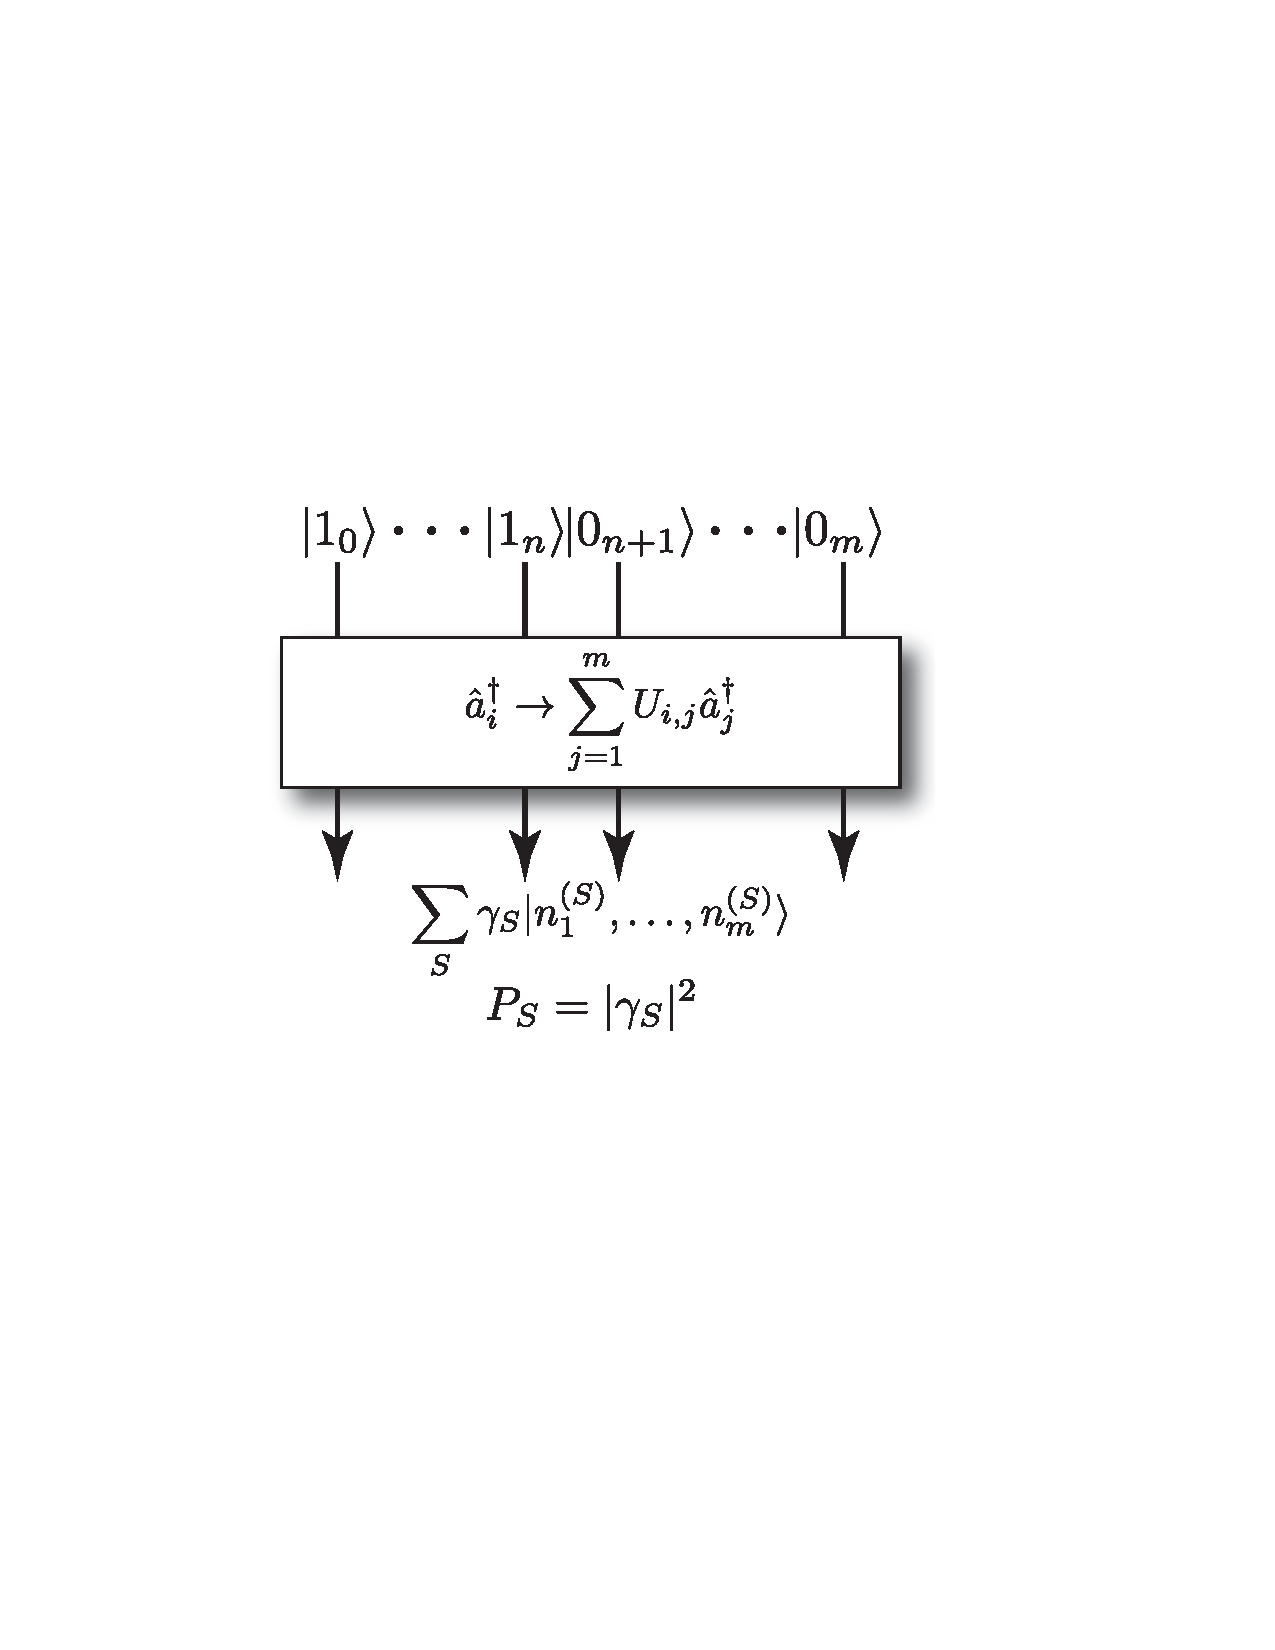
\includegraphics[width=0.7\columnwidth]{model}
\caption{The boson-sampling model. $n$ single photons are prepared in $m$ optical modes. These are evolved via a passive linear optics network $\hat{U}$. Finally the output statistics are sampled via coincidence photodetection. The experiment is repeated many times, reconstructing the output distribution $P_S$.} \label{fig:model}
\end{figure}

It was shown by Scheel \cite{bib:Scheel04perm} that the amplitudes $\gamma_S$ are related to matrix permanents,
\begin{equation}
\gamma_S = \frac{\mathrm{Per}(U_S)}{\sqrt{n_1^{(S)}!\dots n_m^{(S)}!}},
\end{equation}
where $U_S$ is an \mbox{$n\times n$} sub-matrix of $U$, and \mbox{$\mathrm{Per}(U_S)$} is the permanent of $U_S$.

Let us examine this relationship with the permanent more closely. Consider Fig.~\ref{fig:two_photon_perm}. Here the first two modes have single photons, with the remaining modes in the vacuum state. Let us consider the amplitude of measuring one photon at output mode 2 and another at output mode 3. Then there are two ways in which this could occur. Either the first photon reaches mode 2 and the second mode 3, or vice versa, i.e the photons pass straight through, or swap. Therefore there are \mbox{$2!=2$} ways in which the photons could reach the outputs. Thus, this amplitude may be written as,
\begin{eqnarray} \label{eq:coinProbEx}
\gamma_{\{2,3\}} &=& \underbrace{U_{1,2}U_{2,3}}_{\mathrm{walkers\ don't\ swap}} + \underbrace{U_{1,3}U_{2,2}}_{\mathrm{walkers\ swap}} \nonumber \\
&=& \mathrm{Per} \left[ {\begin{array}{cc}
   U_{1,2} & U_{2,2} \\
   U_{1,3} & U_{2,3} \\
  \end{array} } \right],
\end{eqnarray}
which is a \mbox{$2\times 2$} matrix permanent.

\begin{figure}[!htb]
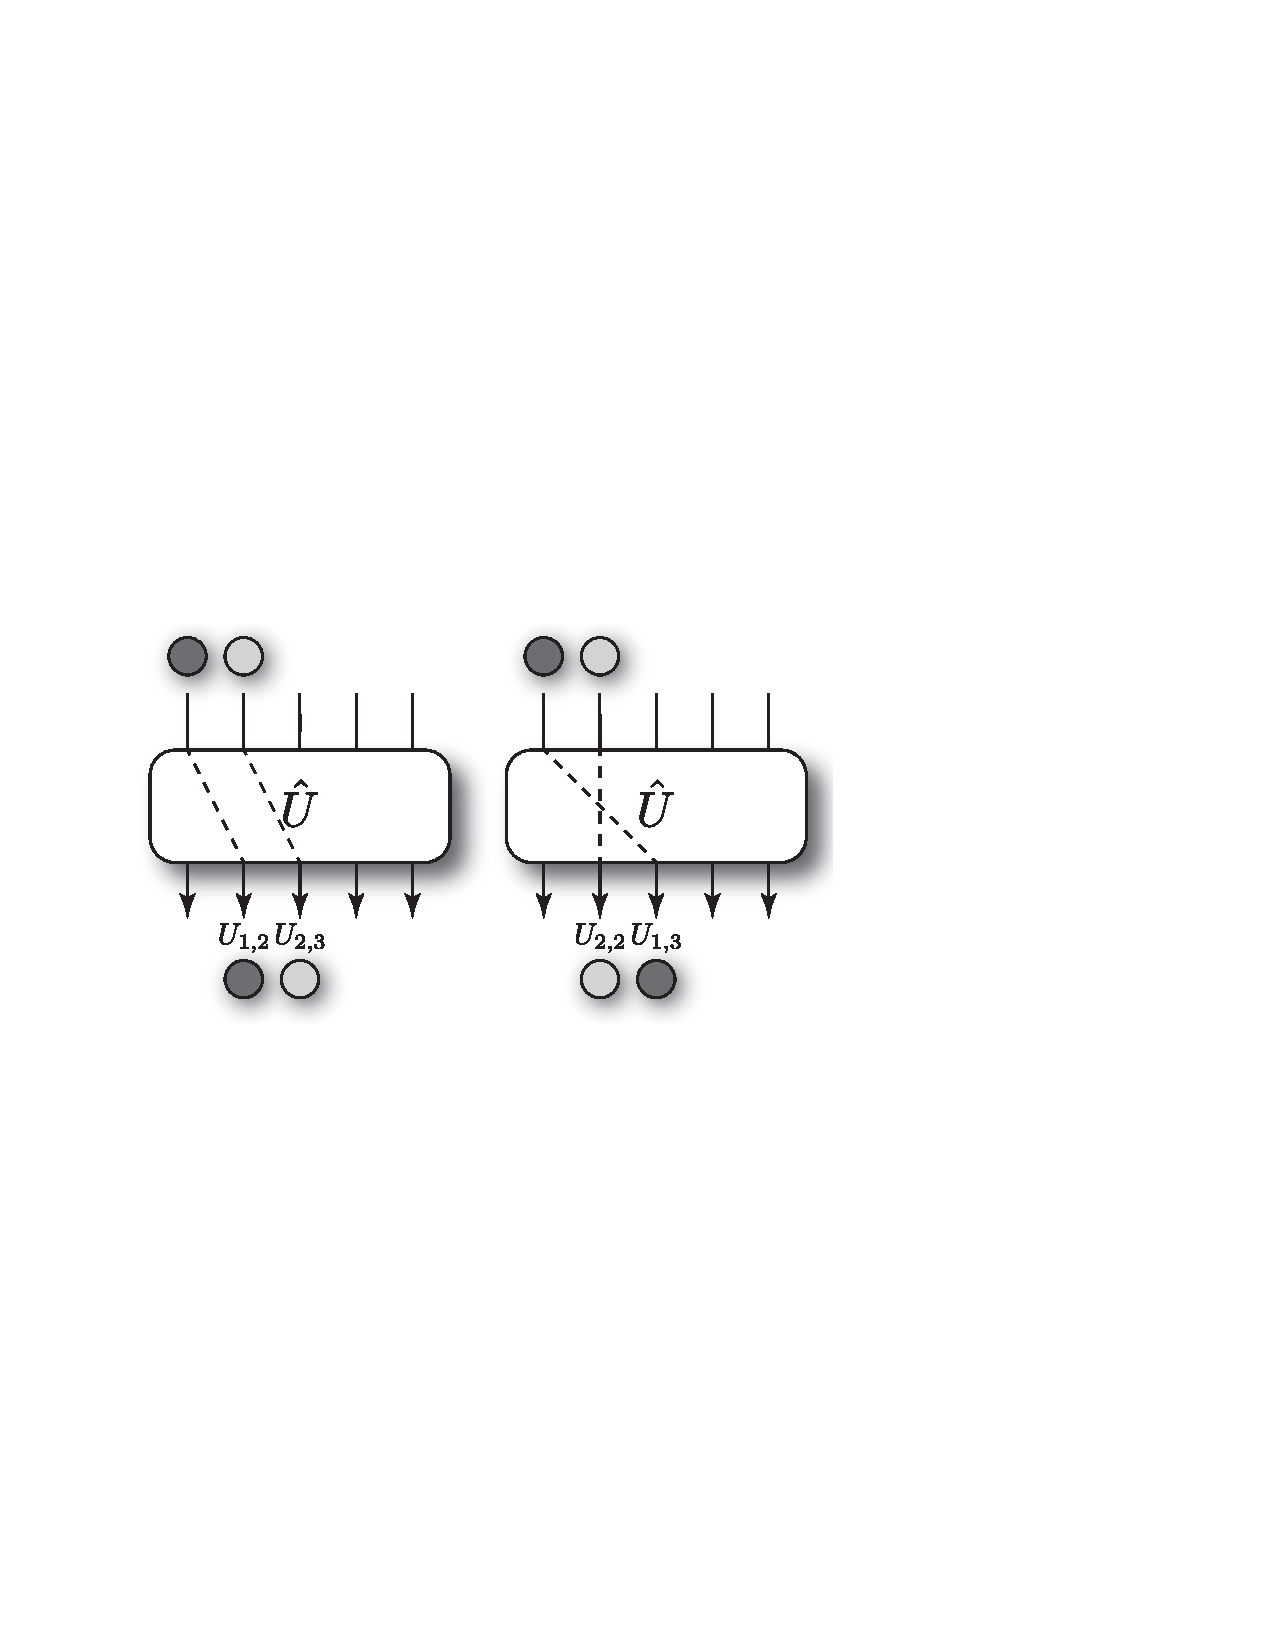
\includegraphics[width=0.7\columnwidth]{two_photon_combinatorics}
\caption{Two-photon boson-sampling, where we wish to calculate the amplitude of measuring a photon at each of the output modes 2 and 3. There are two ways in which this may occur -- either the photons pass straight through, or swap, yielding a sum of two paths.} \label{fig:two_photon_perm}
\end{figure}

As a slightly more complex example, consider the three photon case shown in Fig.~\ref{fig:three_photon_perm}. Now we see that there are \mbox{$3!=6$} ways in which the three photons could reach the outputs, and the associated amplitude is given by a \mbox{$3\times 3$} matrix permanent,
\begin{eqnarray} \label{eq:coinProbEx3}
\gamma_{\{1,2,3\}} &=& U_{1,1}U_{2,2}U_{3,3} + U_{1,1}U_{3,2}U_{2,3} \nonumber \\
&+& U_{2,1}U_{1,2}U_{3,3} + U_{2,1}U_{3,2}U_{1,3} \nonumber \\
&+& U_{3,1}U_{1,2}U_{2,3} + U_{3,1}U_{2,2}U_{1,3}
\nonumber \\
&=& \mathrm{Per} \left[ {\begin{array}{ccc}
   U_{1,1} & U_{2,1} & U_{3,1} \\
   U_{1,2} & U_{2,2} & U_{3,2} \\
   U_{1,3} & U_{2,3} & U_{3,3} \\
  \end{array} } \right].
\end{eqnarray}

\begin{figure}[!htb]
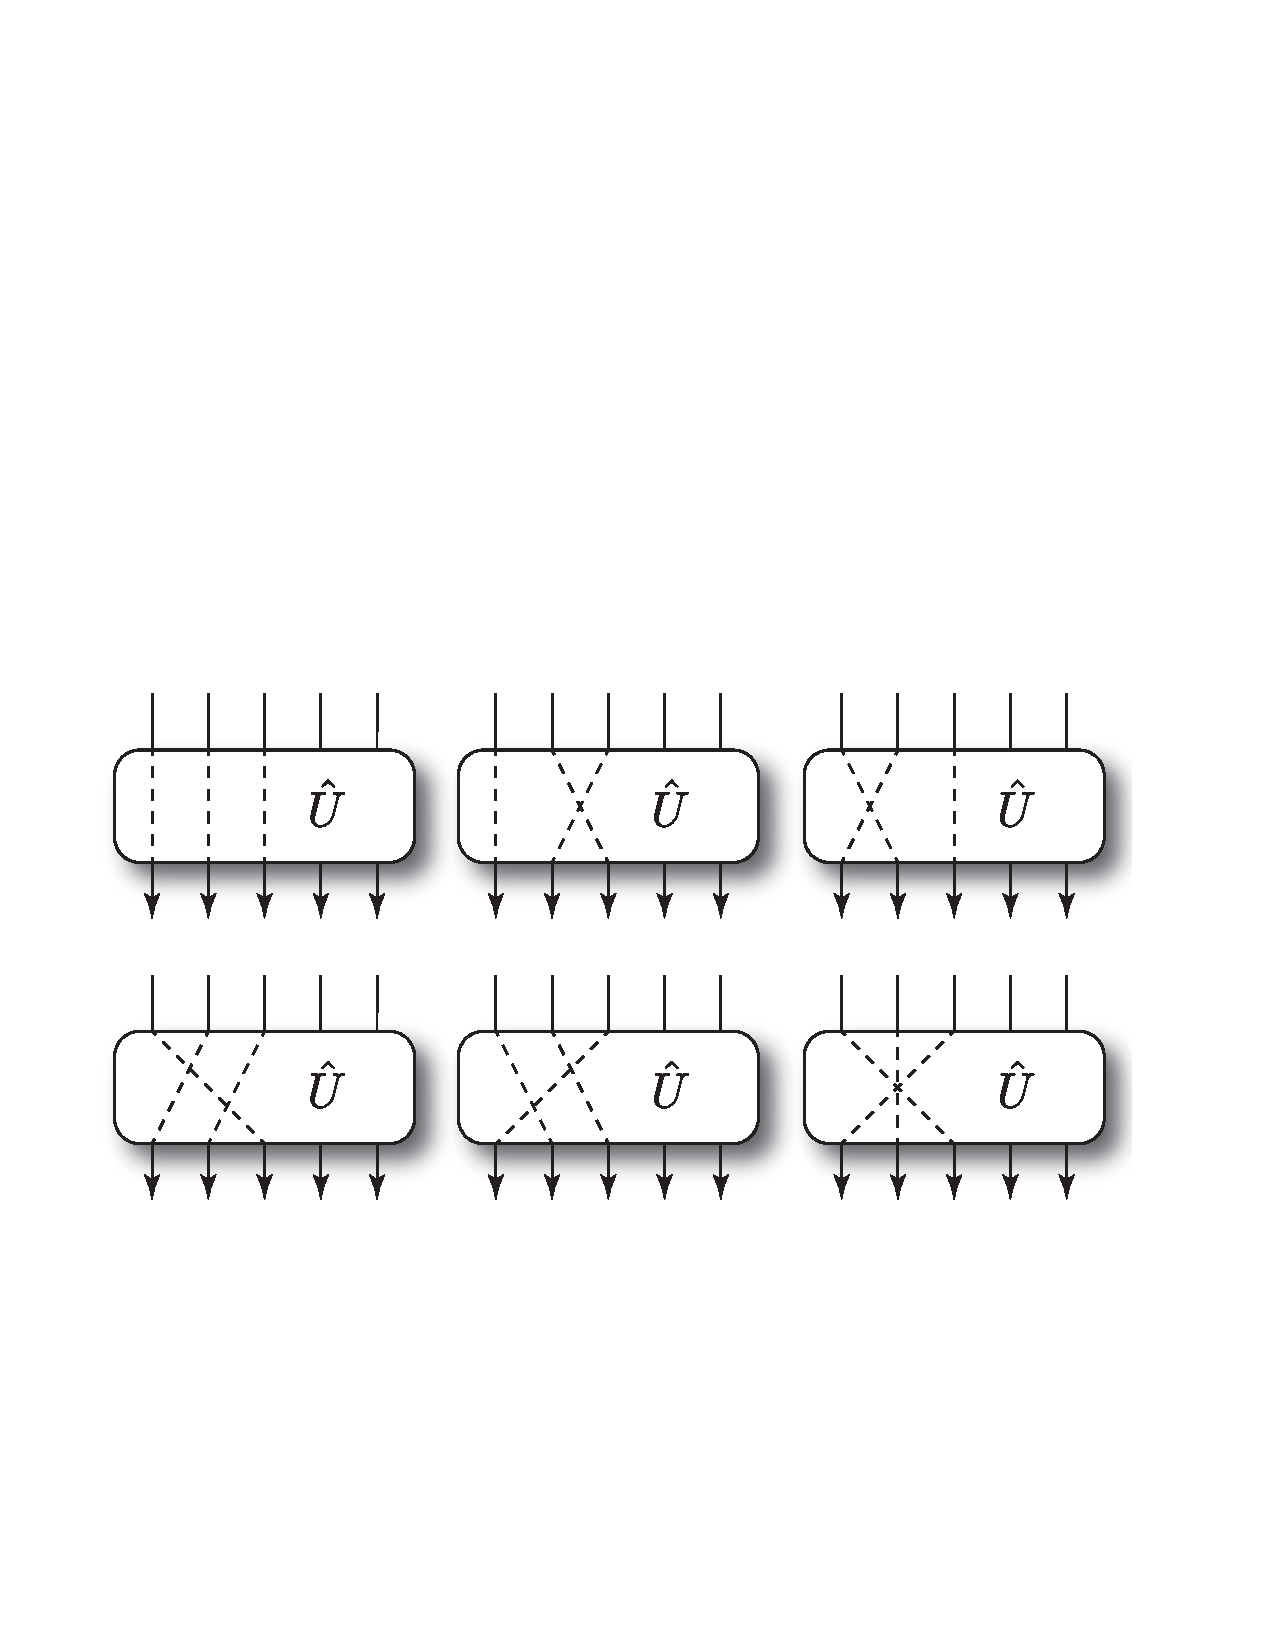
\includegraphics[width=\columnwidth]{three_photon_combinatorics}
\caption{Thee photon boson-sampling, where we wish to calculate the amplitude of measuring a photon at each of the output modes 1, 2 and 3. There are now \mbox{$3!=6$} possible routes for this to occur.} \label{fig:three_photon_perm}
\end{figure}

In general, with $n$ photons, there will be $n!$ ways in which the photons could reach the outputs (assuming they all arrive at distinct outputs), and the associated amplitude will relate to an \mbox{$n\times n$} matrix permanent. Calculating matrix permanents is known to be \textbf{\#P}-complete, even harder than \textbf{NP}-complete, and the best known algorithm for calculating matrix permanents is by Ryser \cite{bib:Ryser63}, requiring \mbox{$O(2^n n^2)$} runtime. Thus, we can immediately see that if boson-sampling were to be classically simulated by calculating the matrix permanents, it would require exponential classical resources.

Because the number of modes scales quadratically with the number of photons, for large systems we are statistically guaranteed that all photons will arrive at different output modes. This implies that in this regime on/off (or `bucket') detectors will suffice, and photon-number resolution is not necessary, a further experimental simplification compared to full-fledged LOQC.

The number of configurations in the output modes scales as,
\begin{equation}
|S| = \binom{n+m-1}{n},
\end{equation}
which is exponential is $n$. Thus, with an `efficient' (i.e sub-exponential) number of trials, we are unlikely to sample from a given configuration more than once. This implies that we are unable to determine any given $P_S$ with more than binary accuracy. Thus, boson-sampling does \emph{not} let us \emph{calculate} matrix permanents, as doing so would require determining amplitudes with a high level of precision, which would require an exponential number of measurements.

The experiment is repeated may times, each time performing a coincidence photodetection at the output modes. Thus, after each run we sample from the distribution $P_S$. This yields a so-called \emph{sampling problem}, whereby the goal is to sample a statistical distribution using a finite number of measurements. This is in contrast to well-known \emph{decision problems}, such as Shor's algorithm \cite{bib:Shor97}, which provide a well-defined answer to a well-posed question.

This sampling problem was shown by AA to be a computationally hard problem. That is, reconstructing the statistical distribution at the output to the boson-sampling device is computationally hard. However, whilst shown to be computationally hard, no known applications for boson-sampling have been described. Thus, boson-sampling acts as an interesting proof-of-principle demonstration that linear optics can outperform classical computers, but, based on present understanding, does not solve a problem of practical interest.

\subsection{Sampling problems vs. decision problems (Peter)}

\subsection{Why is boson-sampling so much easier than linear optics quantum computing? (Peter)}

\subsection{Errors in boson-sampling (Johnny)}
Discuss the 1/poly(n) bound

\section{Boson-sampling and the Extended Church-Turing thesis}

Any model for quantum computation is subject to errors of some form. In the conventional circuit model, this includes errors such as dephasing. In linear optics, this includes photon loss and mode-mismatch. Let us consider a very generic error model for boson-sampling, where the single-photon states are the desired single photon with probability $p$, otherwise are in some erroneous state \cite{bib:BSECT}. This erroneous state could, for example, comprise terms with the wrong photon number (such as loss or second order excitations), or mode-mismatch. Then our input state is of the form,
\begin{equation} \label{eq:error_model}
\hat\rho_\mathrm{in} =\left(\bigotimes_{i=1}^n[p\ket{1}\bra{1} + (1-p)\hat\rho_\mathrm{error}^{(i)}]\right) \otimes [\ket{0}\bra{0}]^{\otimes^{m-n}},
\end{equation}
where \mbox{$\hat\rho_\mathrm{error}^{(i)}$} may be different for each input mode $i$. This is an independent error model, whereby each state is independently subject to an error channel. $p$ stipulates the fidelity of the single photon states. When \mbox{$p=1$}, the states are perfect single photons, and when \mbox{$p<1$}, the state contain erroneous terms. We desire to sample from the distribution of Eq.~\ref{eq:input_state}, whereby none of the input states are erroneous. This occurs with probability $p^n$.

Let $P$ be the probability that upon performing boson-sampling we have sampled from the correct distribution, otherwise we sample from noise. The complexity proof provided by AA only considered the regime where \mbox{$P>1/\mathrm{poly}(n)$}. Thus, for computational hardness, we require \mbox{$p^n > 1/\mathrm{poly}(n)$}. Clearly in the asymptotic limit of large $n$, this bound can never be satisfied for any $p<1$. Thus, with this independent error model, boson-sampling will always fail in the asymptotic limit.

Numerous authors \cite{bib:Broome20122012, bib:ShenDuan13, bib:AA13response, bib:Shchesnovich13, bib:Molmer13} have claimed that large-scale demonstrations of boson-sampling could provide elucidation on the validity of the Extended Church-Turing (ECT) thesis -- the statement that any physical system may be efficiently simulated on a Turing machine. However, it must be noted that the ECT thesis is by definition an asymptotic statement about arbitrarily large systems. Because the required error bound for boson-sampling is never satisfied in this limit, it is clear that boson-sampling cannot elucidate the validity of the ECT thesis as asymptotically large boson-sampling devices must fail under an independent error model.

This concern might be overcome in the future with either (1) a loosing of the error bound to $1/\mathrm{exp}(n)$, or (2) the development of fault-tolerance techniques for boson-sampling. However, to-date no such developments have been made. Thus, based on \emph{present} understanding, boson-sampling will not answer the question as to whether the ECT thesis is correct or not. However, this is distinct from the question `will boson-sampling yield \emph{post-classical} computation?'. The answer to this question may very well be affirmative, as this only requires a finite sized device, just big enough to beat the best classical computers.

\section{Boson-sampling with other classes of quantum optical states (Johnny)}

\section{How to build a boson-sampling device}

In this section we explain the basic components required to build a boson-sampling device. This device consists of three basic components: (1) single-photon sources; (2) linear optics networks; and, (3) photodetectors. Each of these present their own engineering challenges. There are a range of technologies that could be employed for each of these components. However, although boson-sampling is much easier to implement than full-scale LOQC, it remains challenging to build a post-classical boson-sampling device. 

\subsection{Photon sources}

\textbf{add in citations}

The first engineering challenge is to prepare an input state of the form of Eq.~\ref{eq:input_state}. This state may be generated using various photon source technologies. For a review of many of the photon sources see Ref.~\cite{bib:SourceAndDetectorReview}. Presently, the most commonly employed photon source technology is spontaneous parametric down conversion (SPDC).

The SPDC source works by first pumping a non-linear crystal with a laser source. With some probability one of the laser photons interacts with the crystal and emits an entangled superposition of photons across two output modes, the \emph{signal} and \emph{idler}. The output of an SPDC source is of the form,
\begin{equation} \label{SPDC}
\ket{\Psi_\mathrm{SPDC}} = \sqrt{1-\chi^2}\sum_{n=0}^{\infty}\chi^n\ket{n}_s\ket{n}_i,
\end{equation}
where $\chi$ is the squeezing parameter, $n$ is the number of photons, $s$ represents the signal mode, and $i$ represents the idler mode. For boson-sampling, we are interested in the $\ket{1}_s\ket{1}_i$ term of this superposition. The signal photons are measured by a photo-detector and because of the correlation in photon-number, we know that a photon is also present in the idler mode. The idler photons are then routed into one of the input ports of the boson-sampling device using a multiplexer \cite{bib:migdall2002tailoring, bib:LPOR201400027, bib:ma2011experimental}.

There are several problems associated with SPDC sources, which limit the scalability of boson-sampling. The major problem is higher order photon-number terms. In the boson-sampling model we only want the $\ket{1}_s\ket{1}_i$ term, which is far from deterministic. The SPDC source is going to emit the zero-photon term with highest probability, with exponentially decreasing higher order terms. If the heralding photodetector does not have unit efficiency, then the heralded mode may contains higher order photon-number terms.

It was recently shown my Motes \emph{et al.} \cite{bib:motes2013spontaneous} that SPDC sources are scalable in the asymptotic limit for boson-sampling. Specifically, if the photodetection efficiency is sufficient to guarantee post-selection at the output of the boson-sampling device with high probability then the heralded SPDC photons also have asymptotically high fidelity. The boson-sampling architecture with multiplexing is shown in Fig.~\ref{fig:multiplexing}. 

\begin{figure}[!htb]
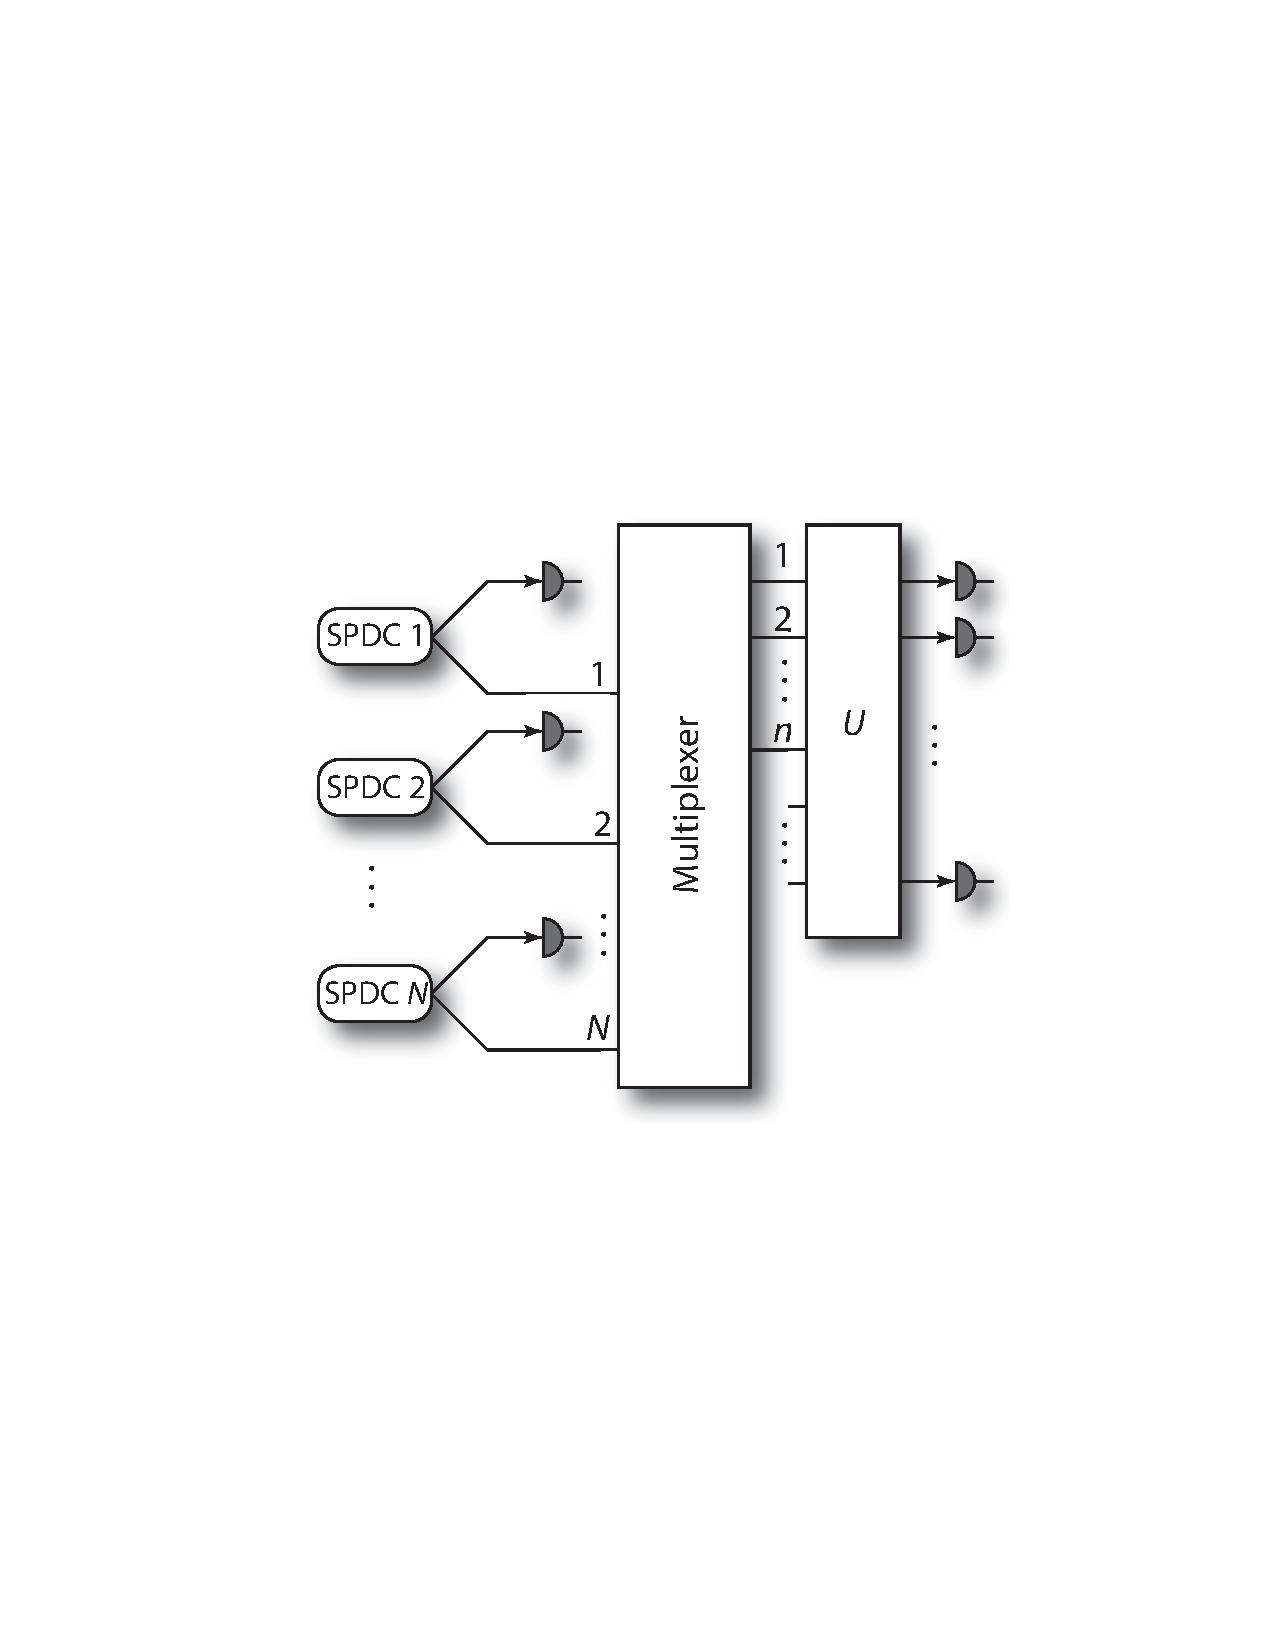
\includegraphics[width=0.7\columnwidth]{multiplexing}
\caption{Boson-sampling architecture using SPDC sources with an active multiplexer. $N$ sources operate in parallel, each heralded by an inefficient single-photon number-resolving detector. It is assumed that \mbox{$N\gg n$}, which guarantees that at least $n$ photons will be heralded. The multiplexer dynamically routes the successfully heralded modes to the first $n$ modes of the unitary network $U$. Finally, photodetection is performed and the output is post-selected on the detection on all $n$ photons.}
\label{fig:multiplexing}
\end{figure}

Another problem is that photons from SPDC sources have uncertainty in their temporal distribution. If a boson-sampling device is built using multiple SPDC sources it is difficult to temporally align each of the $n$ photons entering the device. The error term associated with this scales exponentially with $n$, yielding an error model consistent with Eq.~\ref{eq:error_model}, which undermines operation in the asymptotic limit. 

\subsection{Linear optics networks}

After the input state has been prepared it is evolved via a linear optics network, $\hat{U}$. $\hat{U}$ transforms the input state as per Eq.~\ref{eq:Utransform} and may be completely characterized before the experiment using coherent state inputs \cite{bib:PhysRevLett.73.58}. $\hat{U}$ is composed of an array of discrete elements, namely, beam-splitters and phase-shifters. A beamsplitter with phase-shifters may be represented as a two-mode unitary of the form \cite{bib:GerryKnight05},
\begin{equation} \label{eq:BS}
U_{\mathrm{BS}}(t) = \left( \begin{array}{cc}
e^{i(\alpha-\frac{\beta}{2}-\frac{\gamma}{2})}\mathrm{cos}\left(\frac{\delta}{2}\right) & -e^{i(\alpha-\frac{\beta}{2}+\frac{\gamma}{2})}\mathrm{sin}\left(\frac{\delta}{2}\right)  \\
e^{i(\alpha+\frac{\beta}{2}-\frac{\gamma}{2})}\mathrm{sin}\left(\frac{\delta}{2}\right) & e^{i(\alpha+\frac{\beta}{2}+\frac{\gamma}{2})}\mathrm{cos}\left(\frac{\delta}{2}\right)
\end{array} \right), 
\end{equation}
where \mbox{$0\leq\alpha\leq2\pi$} and \mbox{$0\leq\{\beta,\gamma,\delta\}\leq\pi$} are arbitrary phases. It was shown by Reck \emph{et al.} \cite{bib:Reck94} that an arbitrary unitary $\hat{U}$ can be constructed with $O(m^2)$ optical elements, where $m$ is the number of inputs to the boson-sampling device.

For a $\hat{U}$ that implements a classically hard problem one would need hundreds of discrete optical elements. Constructing an arbitrary $\hat{U}$ using the traditional linear optics approach of setting and aligning each optical element would be extremely cumbersome. Thus, using discrete optical elements is not a very promising route towards scalable boson-sampling.

One method to simplify the construction of the linear optics network is to use integrated waveguides. Quantum interference was first demonstrated with this technology by Peruzzo \emph{et al.} \cite{bib:peruzzo2011multimode}. This technology requires more frugal space requirements, is more optically stable, and far easier to manufacture, allowing the entire linear optics network to be integrated onto a small chip \cite{bib:Politi02052008, bib:matthews2009, bib:Politi04092009}. The main issue with integrated waveguides is achieving sufficiently low loss rates inside of the waveguide and in the coupling of the waveguide to the photon-sources and photo-detectors. Presently, the loss rates in these devices are extremely high and post-selection upon $n$ photons at the output occurs with very low probability. It is foreseeable that photon-sources and photodetectors will eventually be integrated into the waveguide which would eliminate coupling loss rates, substantially improving scalability.   

Another potential route to simplifying the linear optics network is to use time-bin encoding in a loop based architecture \cite{bib:motes2014scalable}. The major advantage of this architecture is that it only requires two delay loops, two on/off switches, and one controllable phase-shifter as shown in Fig.~\ref{fig:fiber_loop}. This possibility eliminates the problem of aligning hundreds of optical elements and has fixed experimental complexity, irrespective of the size of the boson-sampling device. A major problem with this architecture however is that it remains difficult to control a dynamic phase-shifter with high fidelity at a rate that is on the order of the time-bin width $\tau$.

\begin{figure}[!htb]
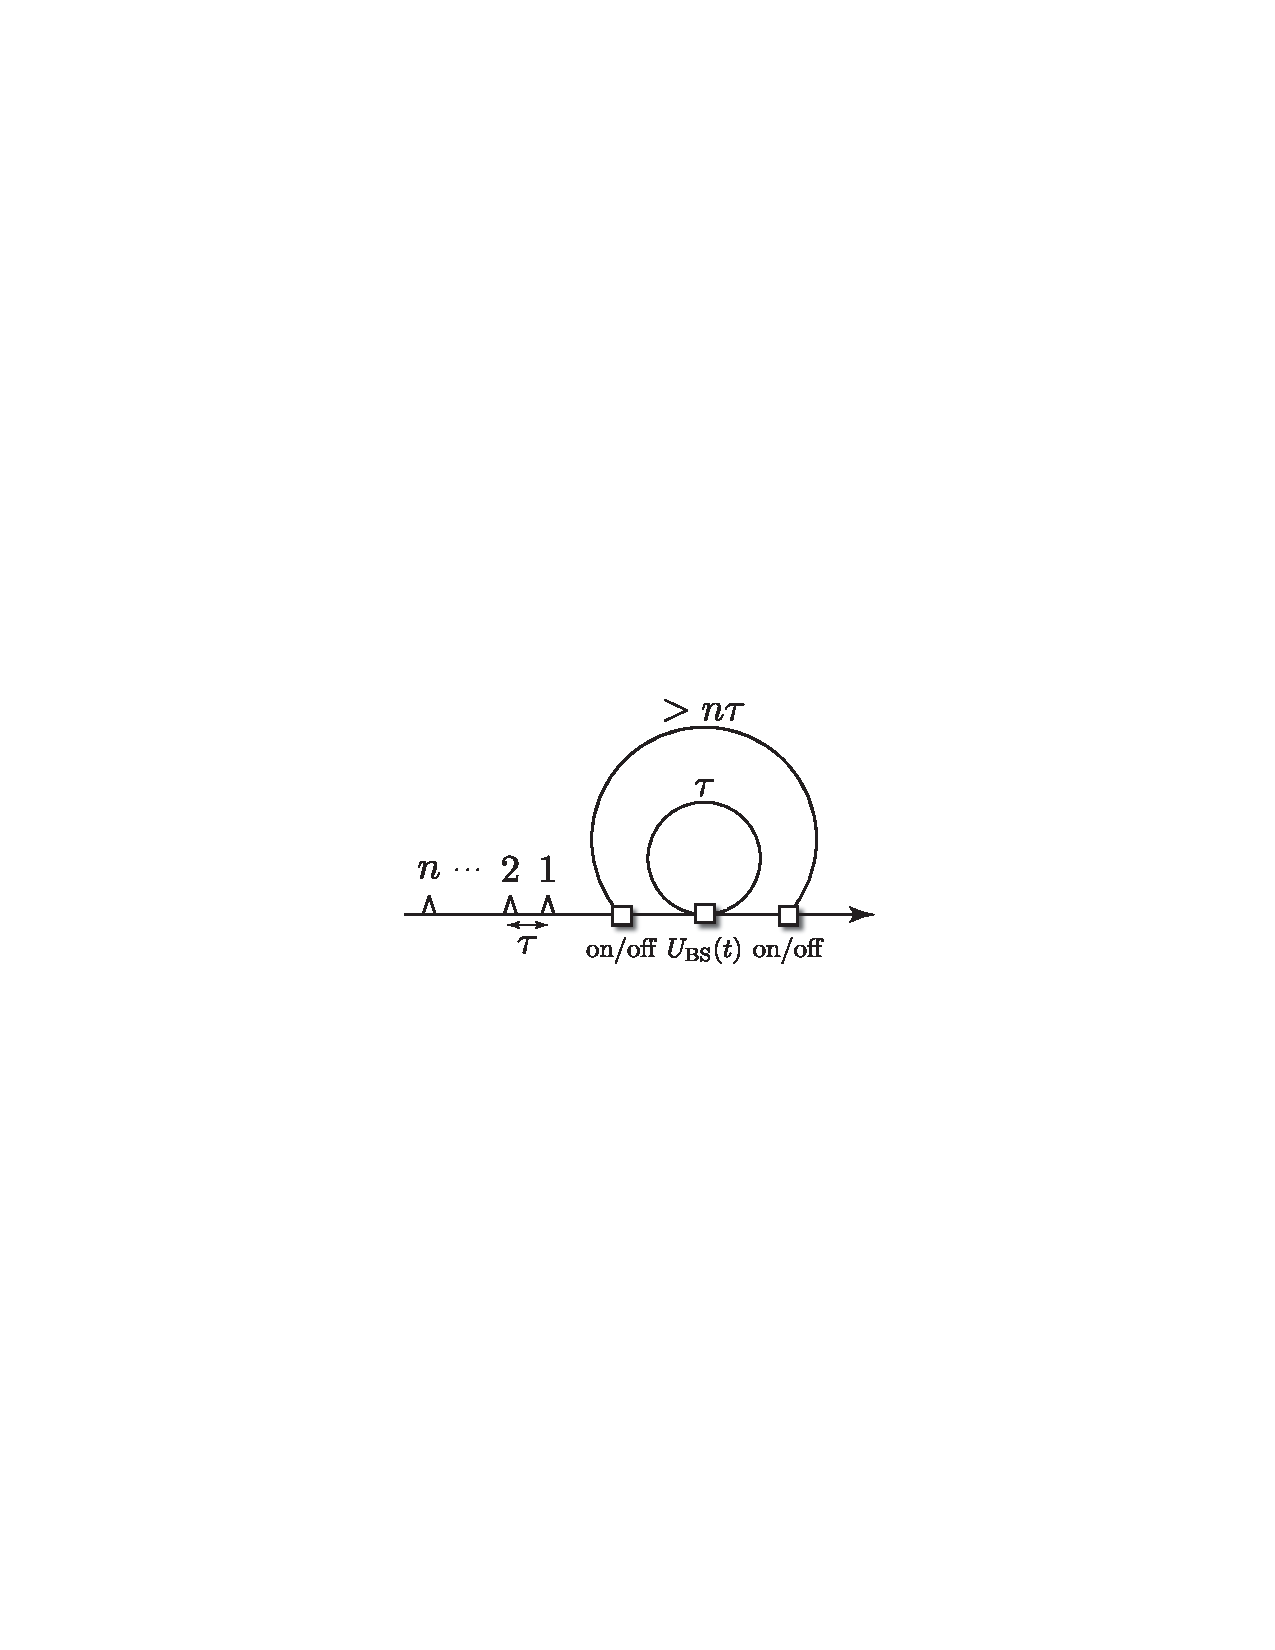
\includegraphics[width=0.7\columnwidth]{fiber_loop}
\caption{Time-bin encoding architecture for implementing a boson-sampling device. Single photons arrive in a train of time-bins instead of in spatial modes. Each time-bin corresponds to spatial modes in the boson-sampling scheme and are separated by time $\tau$. The photon train is coupled into the loop by the first switch. The photons then transverse the inner loop such that each time-bin may interact. The first (last) photon is coupled completely in (out). The outer loop allows an arbitrary number of the smaller loops to be applied consecutively which is determined by the third switch. Finally, the photon train is measured at the output using time-resolved detection.}
\label{fig:fiber_loop}
\end{figure}

\subsection{Photodetection}

The final requirement in the boson-sampling device is sampling the output distribution. With linear optics this is done using photo-detectors. For a review on photodetection see Ref.~\cite{bib:SourceAndDetectorReview}.  

There are two general types of photo-detectors -- photon-number resolving detectors and bucket detectors. The former counts the number of incident photons. These are much more difficult to make and more expensive in general than bucket detectors. Bucket detectors, on the other hand, simply trigger if any non-zero number of photons are incident on the detector.

As discussed earlier, in the limit of large boson-sampling devices, we are statistically guaranteed that we never measure more than one photon per mode, since the number of modes scales as \mbox{$m=O(n^2)$}. Thus, bucket detectors are sufficient for large boson-sampling devices, a significant experimental simplification compared to universal LOQC protocols.

Some of the various types of photo-detectors are:

Number-resolving:

Bucket:


\begin{itemize}
\item List different types of detectors
\item don't need to be number resolving.
\item be sure to describe issues to overcome
\end{itemize}

\section{Conclusion (Jon)}

%
% Acknowledgments
%

\begin{acknowledgments}
This research was conducted by the Australian Research Council Centre of Excellence for Engineered Quantum Systems (Project number CE110001013).
\end{acknowledgments}

%
% Bibliography
%

\bibliography{bibliography}

\end{document}
